% INTRO %
This final section is reserved for explaining the steps on the \textit{implementation stage} and provide some final regards.

% XDP PRIMITVE ACTIONS %
The \textit{Feasibility Test} was fortuitous in exhibiting the environment and tools chosen, allow for the intended demonstration.
Nevertheless, the \textit{feasibility stage} only tackled two primitive actions.
The other three: \textbf{(1)} \textit{XDP\_ABORTED}, \textbf{(2)} \textit{XDP\_TX}, and \textbf{(3)} \textit{XDP\_REDIRECT}, in addition to extra use cases worth exploring, will be the focus on the \textit{implementation stage}. 

% BENCHMARKING %
Although benchmarking was not part of the current paper's proposal, it will be a central point in the next report.
It will only regard the primitive cases and will be preformed through a mix of \textit{XDP} specific structures\cite{XDP} and software developed exclusively to benchmark them, making possible to count the packets processed and express it through time ratios.

% ROADMAP %
\begin{figure}[h]
    \centering
    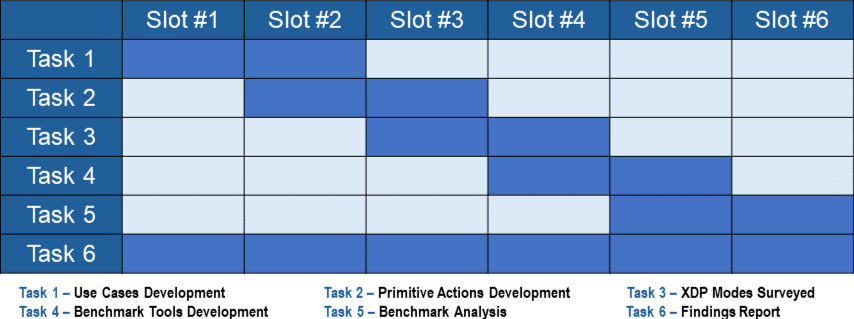
\includegraphics[width=250pt]{src/figures/roadmap.png}
    \caption{Gantt chart disclosing tasks per fixed time slots}
    \label{fig:roadmap}
\end{figure}

% FINAL REGARDS %
The \textit{Feasibility Test} yielded positive results, creating a safe foundation to expand upon the next stage.
During this paper's development, challenges regarding the \textit{XDP} modes were also clarified so new measures could be erected to mitigate them.